\subsection{\textbf{RQ3:} Do developer tools meet developer needs for merge conflicts?}\label{RQ3}
Good merge conflict resolution tools enable practitioners by providing them with reliable information, ease of use, and understandable presentation of information. In order to understand the need for toolset improvements, we asked interview participants open-ended questions about their merge conflict resolution process.

Our interviews informed survey questions ranking 6 practitioner needs for tool improvements and received 119 responses using a 5-point Likert scale to indicate the usefulness each type of tool improvement (1 being \textit{Not Useful}, 3 being \textit{Moderately Useful}, and 5 being \textit{Essential}).

To get a picture of the kinds of tools being used, we asked participants which tools they use during conflict resolution. We received 105 different tools from 115 responses, though some were general responses such as \textit{``my text editor''}. Table~\ref{survey_toolset} lists the top 10 tools used by participants to resolve merge conflicts.

\todo{rough transition, number of survey responses}
\todo{functional deficiencies -> functions not supported by tools, they should all be terms or all be definitions}

\subsubsection{\underline{Information Presentation}}
Complaints about information presentation are a result of bad or inconsistent tool design. For instance, some complaints about inconsistent terminology, coloring, and organization across different resolution tools required developers to reorient themselves within each tool when switching contexts. While these are problems with the way these tools work together, individual tool usability was also questioned. For instance, one survey participant says, 
\begin{displayquote}
\textit{``Tools don't make it easy to work with two arbitrary revisions side by side.''}
\end{displayquote}

\todo{Use the same terms from survey, not toolset fragmentation}
\todo{"Big bang up front"}
\subsubsection{\underline{Toolset Fragmentation:}} Toolset fragmentation was a complaint when participants tried to track down information because they felt that information should be communicated better between different parts of their process. For instance, P1 says, 

\begin{displayquote}
\textit{``I had to jump around between tools and copy and paste version numbers from one to... See, this is why [toolset] integration matters.''}
\end{displayquote}

This frustration is understandable for developers whose workflows frequently get interrupted by tool switches. Psychology studies~\cite{Meiran2000}\cite{gopher2000switching} have found that task switching comes with a cost, and Gerald Weinberg has discussed the problem within engineering teams~\cite{Weinberg1992}. However, when asked, \textit{``How often do you find that having multiple tools has been a problem in your development workflow?''}, 121 survey participants responded with an average response of 2.04 (\textit{Rarely}) on a 5-point Likert scale from \textit{Never} to \textit{Always}. 

To ensure that these developer perceptions were not biased based on the current toolset of the developer (i.e. people do not have a problem with having too many tools because they use IDEs), we compared the tool list for people who chose \textit{Never} or \textit{Rarely} and found that the groups share 9 of the top 10 tools. The fact that developers do not mind using multiple tools suggests that the benefits of a more modular toolset offsets the cost of switching tools with more features or better user experiences in the tools in their toolchains. 

\begin{table}[!]
\renewcommand{\arraystretch}{1.3}
\caption{How much software practitioners trust their merging, history exploration, and/or conflict resolution tools}
\label{survey_tool_trust}
\centering
\begin{tabularx}{0.45\textwidth}{@{}r|*{10}{C}c@{}}
\toprule
Trust Level & Response Count & Response \%\\
\midrule
Completely & 20 & 17\\
A lot & 50 & 41\\
A moderate amount & 41 & 34\\
A little & 10 & 8\\
Not at all & 0 & 0\\
\bottomrule
\end{tabularx}
\end{table}

\subsubsection{\underline{Tool Mistrust:}}
Tool mistrust seemed to come from being unsure about what the tool was really doing. Many merging tools obscure the steps that are actually being taken, making developers hesitant to trust that the appropriate steps have been initiated by the tool. 
\begin{displayquote}
\textit{``I've never trusted the merge tools, in a way. Or the diff tools. It would always just make me skittish. So my overall perception is that I'm scared of them. Sometimes I'll even manually go and do the merge myself rather than use a tool. Just because I've had several times where it's a bad merge, and I broke some code.''}
\end{displayquote}
This quote comes from P4, a software developer with 10 years of experience.
This prompted us to ask developers how much they trust thier merging, history exploration, and/or conflict resolution tools. Of 121 respondents to this question, 91.74\% said that they trusted their tools at least \textit{A moderate amount}, and 57.86\% said they trust their tools \textit{A lot} or \textit{Completely} (Table \ref{survey_tool_trust}). This raises the questions: 
\begin{itemize}
\item How much tool trust is enough? 
\item What is the trust threshold for not using a tool anymore?
\end{itemize}
If we consider this problem conservatively, nearly 1 in 10 software practitioners are using tools that they cannot trust (see Table~\ref{survey_tool_trust}). Since no previous work exists relating to minimum acceptable levels of trust in a toolset, it is possible that up to 42.1\% of developers (those with \textit{A moderate amount} of trust or less) operate within this gap in tool trust.

As seen in Sections \ref{RQ1} and \ref{RQ2}, developers mentioned both size and complexity in the interviews, which raised questions about how developers view each of these metrics. More specifically, we wanted to know how well developers think tools support increased size and complexity.  
This motivated a survey question to compare increased size to increased complexity by asking participants to rate how well their tools handle the following kinds of conflicts:

\begin{itemize}
	\item Simple, small merge conflict resolutions
	\item Simple, large merge conflict resolutions 
	\item Complex, small merge conflict resolutions
	\item Complex, large merge conflict resolutions
\end{itemize}

Our results show that current tools handle increasing the size of the conflict better than increasing the complexity of the conflict. This trend was seen across all experience levels, as visualized in Figure \ref{size_vs_complexity}.

\begin{figure*}[!t]
\centering
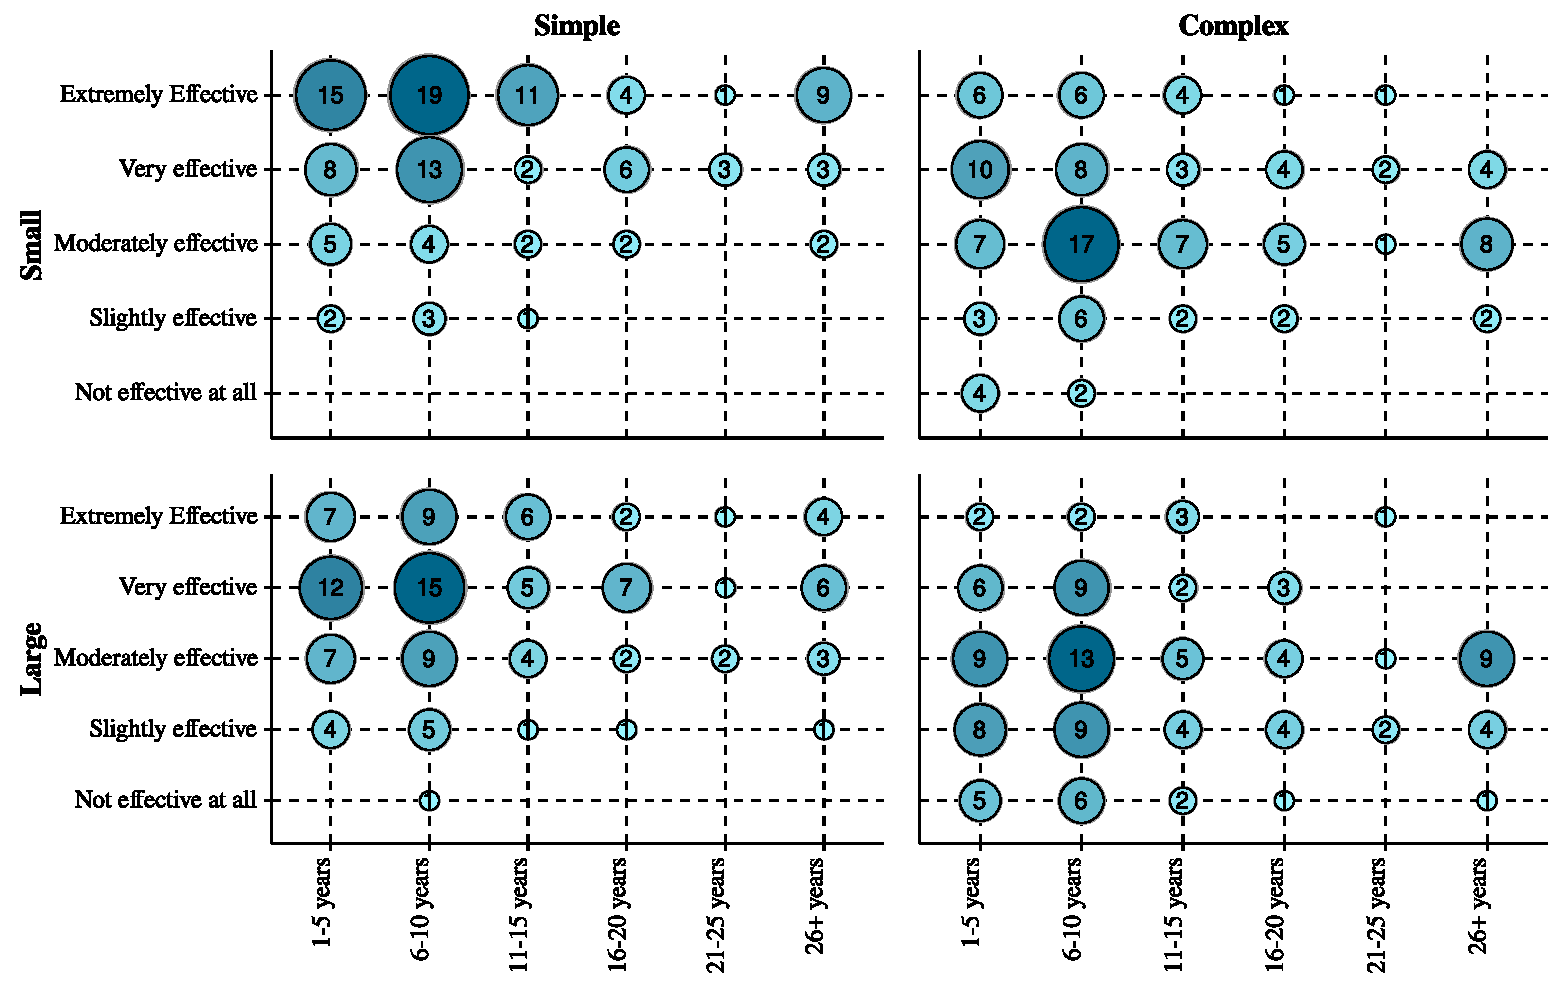
\includegraphics[width=\textwidth]{ConflictComplexityVsSize.pdf}
\caption{Effectiveness of developer tools in supporting varying levels of size and complexity (by developer experience). Values are number of responses per answer, and bubble size indicates the number of responses for comparison purposes.}
\label{size_vs_complexity}
\end{figure*}

\subsubsection{\underline{History Exploration:}}
Notably, many tool-related complaints in the interviews came from within the context of the \textit{Archeology Lens}~\cite{mihai_lenses}, meaning that developers find tool support lacking when trying to explore older history to understand the evolution of a project or even a single line of code. In the words of P1, 

\begin{displayquote}
\textit{``Give me a way to explore the history. To drill down, to go back up, you know? To resurface and understand what happened.''}
\end{displayquote}

The reality for developers using Git for more advanced history exploration use cases is that tool support is thin. P1, as someone who frequently dives deep into Git history, had resorted to writing his own scripts to better find the parts of the history that he really cares about. P9 described a similar tool developed by their open-source project which fills the need for more advanced branch diffing:
\begin{displayquote}
\textit{``git-diff will just do the diff based on the SHAs... we're adding metadata and cherry picking, [so] the SHAs are always going to be changing... this actually allows us to do a comparison based on SHA but then fall back to author and commit title and metadata information... It also hooks into GitHub labels and uses the labels on the project to do some more advanced heuristics.''}
\end{displayquote}

P9 says that all of these changes are in an attempt to create something that will \textit{``essentially create a true diff''.}
This suggests that current tools have not been able to keep up with the rapid expansion of metadata that Git and Github are able to provide, to the extent that projects will divert resources to create a tool for more advanced diffing functionality. 

\subsubsection{\underline{Tool functional deficiencies}}
When told that our study was seeking to find difficulties in resolving merge conflicts, some participants prepared examples of functional deficiencies in conflict resolution tools. P3 shared a specific case from a backporting~\cite{gutzmann2009backporting} experience. In a large system, it is extremely hard to understand when code was deleted. The \texttt{--reverse} option for the \textit{Git Blame} tool offers this functionality, but as P3 points out:  

\begin{displayquote}
\textit{``It still requires thorough background knowledge of the code base. Also I work on large changes in time in hot paths. This could mean many additions and deletions that would lead to further confusion.''}
\end{displayquote}

 This illustrates the case of a tool that performs well in most cases but does not scale well to larger and more complex codebases.
 
 P1 mentions a specific issue that he encounters to illustrate that tools work with a shallow understanding of a merge conflict's process. He describes a conflict where one branch cherrypicks changes from the other, then the second branch reverts the same changes that were cherrypicked. When the two branches merge back together, tools have trouble supporting the resolution of the more complex conflict:
 \begin{displayquote}
 \textit{``So cherrypick on one branch, revert on the other, equals disaster. Most tools... just do three-way branch because they limit their vision to those three parts. They don't try to understand the actual scenario.''}
 \end{displayquote}
 Using this in light of our top difficulties from Table \ref{survey_res_diffs} suggests that tools would benefit from assisting developers in more complex situations by providing them with more specific information about what caused the conflict (in this case, the combination of cherrypicking and reverting).

\begin{table}[!]
\renewcommand{\arraystretch}{1.3}
\caption{Survey Participant Toolset (Top 10 tools)}
\label{survey_toolset}
\centering
\begin{tabularx}{0.45\textwidth}{@{}r|*{10}{C}c@{}c@{}}
\toprule
Tool & \# Participants & Description\\
\midrule
Git	& 37 & Version Control System\\
Vim/vi & 17 & Text Editor\\
Text Editor (unspecified) & 14 & Text Editor\\
Git Diff & 11 & Diffing Tool\\
GitHub & 11 & Website\\
Eclipse & 10 & IDE\\
KDiff3 & 9 & Diff \& Merge\\
Meld & 8 & Diff \& Merge\\
SourceTree & 8 & Git/Hg Desktop Client\\
Sublime Text & 7 & Text Editor\\
\bottomrule
\end{tabularx}
\end{table}